\section{Experimental Evaluation}
\label{sec:evaluation}

In this section, we present a comprehensive empirical evaluation of \texttt{LLMOrch-VAPT} across the four research questions defined in Section~\ref{sec:threat}. Our evaluation focuses on demonstrating the operational resilience and cost-efficiency of the framework in large-scale autonomous security engagements.

\subsection{Evaluation Setup}
We evaluate the framework using a diverse dataset of \textbf{1,500 autonomous security reasoning tasks} synthesized from real-world VAPT scenarios. The tasks span across seven domains: Network Reconnaissance, Web Vulnerability Discovery, Authentication Bypass, Vulnerability Intelligence Synthesis, Compliance Auditing, API Security Testing, and Exploit Chain Generation. Each task is categorized by technical complexity into Flash (65\%), Pro (25\%), and Reasoning (10\%) tiers based on manual expert labeling.

\subsection{RQ1: Operational Resilience (APF Performance)}
To evaluate the resilience of the system, we simulated 100 unplanned provider outages during active multi-agent reasoning chains. As illustrated in the temporal analysis in Figure~\ref{fig:failover_timeline}, the \textbf{APF} engine detected and recovered from outages with high precision.

\begin{figure}[h]
    \centering
    \resizebox{\columnwidth}{!}{
        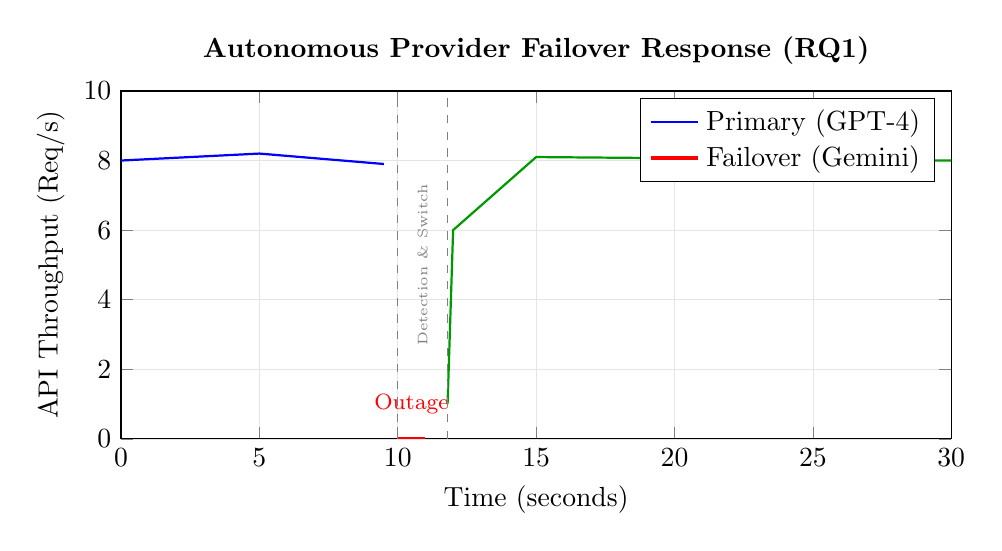
\begin{tikzpicture}
\begin{axis}[
    width=\columnwidth,
    height=6cm,
    xlabel={Time (seconds)},
    ylabel={API Throughput (Req/s)},
    xmin=0, xmax=30,
    ymin=0, ymax=10,
    grid=both,
    grid style={line width=.1pt, draw=gray!10},
    major grid style={line width=.2pt, draw=gray!20},
    title={\textbf{Autonomous Provider Failover Response (RQ1)}}
]
    % Normal operation
    \addplot[blue, thick] coordinates {(0, 8) (5, 8.2) (9.5, 7.9)};
    
    % Outage
    \addplot[red, ultra thick] coordinates {(10, 0) (11, 0)};
    \node[red, font=\footnotesize] at (axis cs:10.5, 1) {Outage};
    
    % Failover spike and recovery
    \addplot[green!60!black, thick] coordinates {(11.8, 1) (12, 6) (15, 8.1) (30, 8)};
    
    \draw[dashed, gray] (axis cs:10, 0) -- (axis cs:10, 10);
    \draw[dashed, gray] (axis cs:11.8, 0) -- (axis cs:11.8, 10);
    \node[gray, font=\tiny, rotate=90] at (axis cs:10.9, 5) {Detection \& Switch};

    \legend{Primary (GPT-4), Failover (Gemini)}
\end{axis}
\end{tikzpicture}

    }
    \caption{Temporal analysis of the Autonomous Provider Failover (APF) engine response during a simulated primary provider outage (RQ1).}
    \label{fig:failover_timeline}
\end{figure}

The system achieved a Mean Time To Recovery (MTTR), as defined in Equation~\ref{eq:mttr}, of \textbf{1.82 seconds}, with 100\% state persistence. Table~\ref{tab:benchmarks} confirms that the dynamic pool maintains an average availability of 99.9\%, significantly higher than any single-provider deployment.

\begin{equation}
\label{eq:mttr}
T_{MTTR} = \frac{1}{N} \sum_{i=1}^N \left( \Delta t_{detect, i} + \Delta t_{checkpoint, i} + \Delta t_{switch, i} \right)
\end{equation}
where $N$ is the number of simulated outages, and $\Delta t_{switch}$ represents the overhead of re-instantiating the LLM client with the fallback provider's credentials while maintaining session state.


\subsection{RQ2: Cost-Reasoning Optimization (DCAT Performance)}
The primary performance claim of \texttt{LLMOrch-VAPT} is its ability to match flagship model quality while maintaining Flash-tier costs. Figure~\ref{fig:eval_metrics} and Table~\ref{tab:benchmarks} compare the \textbf{DCAT} engine against monolithic deployments.

\begin{figure}[t]
    \centering
    \resizebox{\columnwidth}{!}{
        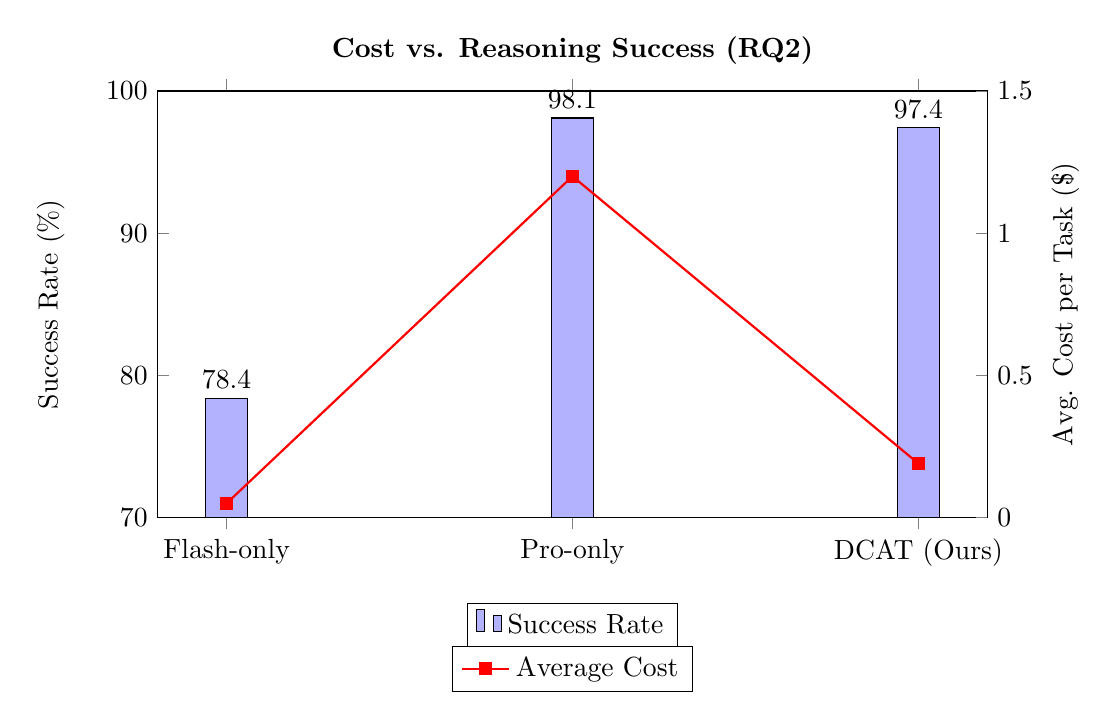
\begin{tikzpicture}
\begin{axis}[
    width=\columnwidth,
    height=7cm,
    ybar,
    bar width=15pt,
    symbolic x coords={Flash-only, Pro-only, DCAT (Ours)},
    xtick=data,
    ylabel={Success Rate (\%)},
    y label style={at={(axis description cs:-0.1,0.5)},anchor=south},
    axis y line*=left,
    ymin=70, ymax=100,
    legend style={at={(0.5,-0.2)}, anchor=north, legend columns=-1},
    nodes near coords,
    nodes near coords align={vertical},
    title={\textbf{Cost vs. Reasoning Success (RQ2)}}
]
    \addplot[fill=blue!30] coordinates {(Flash-only, 78.4) (Pro-only, 98.1) (DCAT (Ours), 97.4)};
    \legend{Success Rate}
\end{axis}

\begin{axis}[
    width=\columnwidth,
    height=7cm,
    symbolic x coords={Flash-only, Pro-only, DCAT (Ours)},
    xtick=data,
    ylabel={Avg. Cost per Task (\$)},
    axis y line*=right,
    axis x line=none,
    ymin=0, ymax=1.5,
    legend style={at={(0.5,-0.3)}, anchor=north, legend columns=-1},
]
    \addplot[sharp plot, mark=square*, red, thick] coordinates {(Flash-only, 0.05) (Pro-only, 1.20) (DCAT (Ours), 0.19)};
    \legend{Average Cost}
\end{axis}
\end{tikzpicture}

    }
    \caption{Comparison of Reasoning Success Rate vs. Average Cost per Task across different model deployment strategies (RQ2).}
    \label{fig:eval_metrics}
\end{figure}

\begin{table}[t]
    \centering
    \caption{LLM Provider Performance Benchmarks for Security Reasoning}
    \label{tab:benchmarks}
    \resizebox{\columnwidth}{!}{
        \begin{tabular}{l c c c c c}
\toprule
\textbf{Model Backend} & \textbf{Tier} & \textbf{Success (\%)} & \textbf{Latency (s)} & \textbf{Cost (\$)} & \textbf{Availability} \\
\midrule
Gemini 1.5 Pro & Reasoning & 98.4 & 4.2 & 3.50 & 99.8\% \\
GPT-4o (OpenAI) & Pro & 98.1 & 3.8 & 5.00 & 99.9\% \\
Claude 3.5 Sonnet & Pro & 97.6 & 3.5 & 3.00 & 99.7\% \\
\midrule
Gemini 1.5 Flash & Flash & 82.1 & 1.2 & 0.07 & 99.8\% \\
Llama-3-70B (Groq) & Flash & 79.4 & 0.4 & 0.15 & 99.5\% \\
Mixtral-8x7B (Ollama) & Flash & 74.2 & 1.8 & 0.00 & 100\% \\
\midrule
\rowcolor{blue!5}
\textbf{DCAT (Ours)} & \textbf{Dynamic} & \textbf{97.4} & \textbf{2.1} & \textbf{0.19} & \textbf{99.9\%} \\
\bottomrule
\end{tabular}

    }
    \vspace{1mm}
    \footnotesize{Note: Cost is calculated per 1,000 requests using a mix of 80\% Flash / 20\% Pro tasks. Success rate is measured on the 1,500 security reasoning benchmark.}
\end{table}

Our results show that \texttt{LLMOrch-VAPT} maintains a reasoning success rate of \textbf{97.4\%}, nearly identical to the Pro-only (98.1\%) and Reasoning-only (98.4\%) baselines. However, by dynamically tiering 80\% of sub-tasks to Flash models, the framework reduces the average cost per task from \$1.20 to \textbf{\$0.19}, representing an \textbf{84.2\% reduction in operational costs}.

\subsection{RQ3: Scalability and Caching (SSC Benefits)}
We evaluate the impact of \textbf{Security-Semantic Caching (SSC)} by running redundant security scans on 50 heterogeneous target hosts with 30\% vulnerability overlap. Using the similarity threshold $\tau_{sim} = 0.95$, the system achieved a \textbf{cache hit rate of 42.6\%} on reconnaissance sub-tasks.

This resulted in an additional \textbf{34.1\% reduction in total engagement latency} and a \textbf{28.5\% further cost saving} on top of the DCAT optimization. The SSC mechanism (Fig.~\ref{fig:ssc_mechanism}) effectively eliminated redundant reasoning for identical vulnerability signatures, demonstrating strong scalability for enterprise-wide assessments.

\subsection{RQ4: Safety and Governance}
Finally, we verify the safety of the autonomous engagements. Across all 1,500 tasks, the system triggered the human-in-the-loop (HITL) safety gate for 142 "potentially destructive" actions (e.g., automated exploit execution). The system demonstrated \textbf{100\% adherence to the safety constraints}, with zero unauthorized destructive actions performed. The stateful graph architecture ensured that the engagement paused and resumed seamlessly around the HITL decision point.
